\section{Modellierung}

\begin{defi}{Modell}
    Ein \emph{Modell} ist eine Abstraktion eines Systems, die benutzt wird, um ein existierendes System zu beschreiben oder ein neu zu erstellendes System zu spezifizieren.

    Ein Modell wird so konstruiert, dass es anstelle des Originals für den jeweils gegebenen Zweck verwendet werden kann.

    Eigenschaften eines Modells:
    \begin{itemize}
        \item \emph{Abbildung}: Das Modell stellt ein Abbild des zu untersuchenden Systems dar.
        \item \emph{Reduktion}: Das Modell abstrahiert von irrelevanten Eigenschaften und erleichtert damit die Untersuchung des Systems.
        \item \emph{Pragmatik}: Das Modell ist für den jeweiligen Zweck geeignet.
    \end{itemize}
\end{defi}

\begin{example}{Modell}
    \begin{center}
        \raisebox{-0.5\height}{
\includegraphics[width=.4\textwidth]{includes/figures/example_modell.png}}
        \hspace{6em}
        \raisebox{-0.5\height}{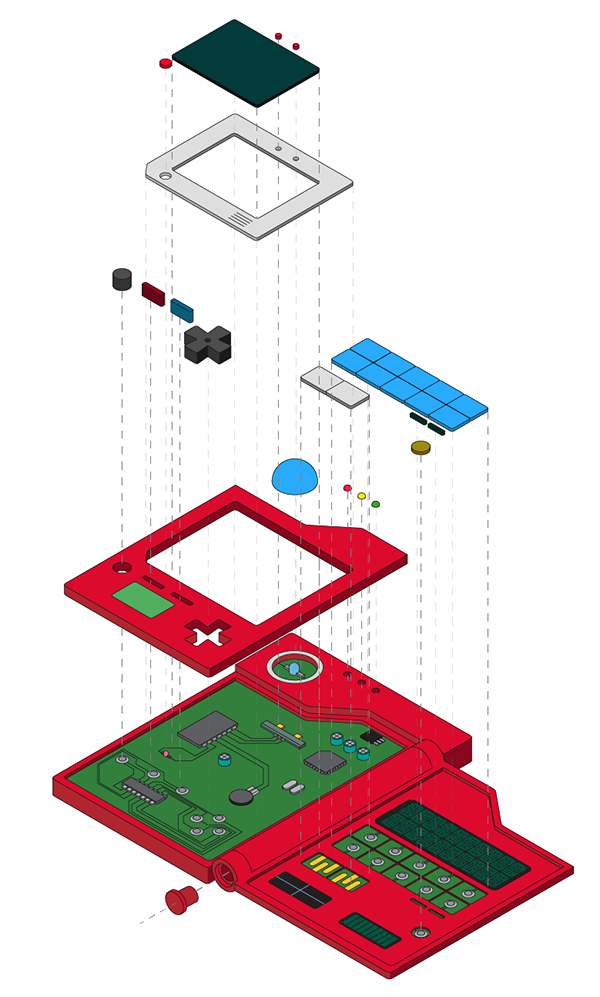
\includegraphics[width=.3\textwidth]{includes/figures/example_modell_2.png}}
    \end{center}
\end{example}

\begin{bonus}{Zweck eines Modells}
    \begin{tabularx}{\textwidth}{|l|X|}
        \hline
        \bfseries Verstehen     & Das Modell erleichtert \emph{mir} durch geeignete Abstraktionen das Verständnis des Systems                                              \\
        \hline
        \bfseries Kommunikation & Das Modell wird dazu verwendet, \emph{anderen Personen} das zugrunde liegende System zu erläutern                                        \\
        \hline
        \bfseries Analyse       & Mit Hilfe des Modells werden \emph{Eigenschaften} des Systems untersucht                                                                 \\
        \hline
        \bfseries Simulation    & Das Modell wird benutzt, um das Verhalten des Systems zu simulieren und dadurch Erkenntnisse über das tatsächliche Verhalten zu gewinnen \\
        \hline
        \bfseries Spezifikation & Das Modell dient als Vorschrift für ein noch zu erstellendes System                                                                      \\
        \hline
        \bfseries Generierung   & Aus dem Modell wird zu erstellende System automatisch erzeugt                                                                            \\
        \hline
    \end{tabularx}
\end{bonus}

\begin{defi}{Präskriptive und deskriptive Modellierung}
    Bei \emph{präskriptiver (vorschreibender) Modellierung} dient das Modell als Spezifikation für die Realisierung (Vorbild).

    Bei \emph{deskriptiver (beschreibender) Modellierung} wird das Modell als Sicht auf ein bereits existierendes System konstruiert (Abbild).
\end{defi}

\begin{defi}{Strukturelles Modell}
    Ein \emph{strukturelles Modell} beschreibt die statische Struktur eines Systems (Elemente und Beziehungen).
\end{defi}

\begin{defi}{Verhaltensmodell}
    Ein \emph{Verhaltensmodell} beschreibt das dynamische Verhalten eines Systems (Ausführung von Operationen, Reihenfolge von Schritten).
\end{defi}

\begin{defi}{Objektorientierte Analyse}
    In der \emph{objektorientierte Analyse} (OOA) geht es darum, die Anforderungen objektorientiert zu erfassen und zu beschreiben, die das zu entwickelnde Softwaresystem erfüllen soll.
    In dieser Phase werden alle Fakten gesammelt, dargestellt und überprüft.
    Dies kann in Form eines textuellen Pflichtenheftes geschehen.

    Ergebnis der objektorientierten Analyse ist ein allgemeines Produktmodell in Form eines objektorientierten Analyse-Modells (OOA-Modell).
    Diese fachliche Beschreibung mit objektorientierten Konzepten enthält verschiedene Artefakte wie Diagramme und Darstellungen von Kontrollstrukturen.
\end{defi}

\begin{defi}{Schritte zum OOA-Modell}
    \begin{enumerate}
        \item Klassen finden
        \item Beziehungen und Aggregationen finden
        \item Klassenkomponenten finden:
              \begin{enumerate}
                  \item Attribute finden
                  \item Externe Operationen finden
              \end{enumerate}
        \item Objekt-Lebenszyklus erstellen
        \item Vererbungsstrukturen finden
        \item Interne Operationen finden
        \item Operationen spezifizieren
        \item Vererbungsstrukturen prüfen
        \item Beziehungen und Aggregationen prüfen
        \item Subsysteme finden
    \end{enumerate}

    Je nach Projektfluss sind auch \emph{Vorgriffe} und \emph{Rückgriffe} oder \emph{Iterationen} denkbar bzw. nötig.

    Neben dem Kern-OO-Modell sollten noch ein \emph{Glossar} und eine \emph{Liste offener Fragen} geführt werden.
\end{defi}

\begin{defi}{Objektorientiertes Design}
    Beim \emph{objektorientierten Design} (OOD) wird das in der objektorientierten Analyse erstellte Domänenmodell weiterentwickelt und darauf aufbauend ein Systementwurf erstellt.
    Dabei wird das allgemeine Modell in eine konkrete Softwarearchitektur umgeformt, die Informationen über Details der technischen Umsetzung enthält und direkt als Vorlage für die Implementierung in einer Programmiersprache dient, die idealerweise objektorientierte Programmierung (OOP) unterstützt.

    Dadurch, dass in den Entwicklungsphasen Analyse und Design bereits objektorientierte Techniken eingesetzt werden, wird der Übergang zur Implementierung in einer objektorientierten Programmiersprache erleichtert.
\end{defi}